\section{Experimental design and results}

\subsection{Dataset Selection}

There are morn than thousands of ambugious words in the SemCor corpuse, by our
definition in secton~\ref{sec:formulate:preprocess}, which will translate to
more than thousands of datasets and the corresponding machine learning tasks.
However, not all dataset is qualified for a tractable machine learning problem. 
The problem is that some words have senses that are rarely appeared in the
sencor corpus, which is typically 1 or 2 appearances.
The lack of data makes the word sense unlearnable.
Therefore, we use two criteria to select the set of training set we use in our
experiment:
(1) Overall instances greate than 200, 
and (2) Each sense ids (labels / classes) appear at least 20 times.

These critia filters out the eight words we use in evaluation
(section~\ref{sec:eval:results}).

\subsection{Parameters Tuning}

\Paragraph{Logistic Regression}
We first perform a parameter search over 5-fold cross-validation over the entire
training set for different words. We tested different regularization values,
solvers, multiclass metrics. Finally we found that in most cases by setting C=1,
solver=``newtown\_cg'', max\_iter = 500, and metric=``multinomial'' we can get
the best accuracy and f1 scores. We'll set them to be the global parameters over
logistic regression classifier for each word. 

\Paragraph{SVM}.
For each type of SVM models, we execute a 3-fold cross-validation on the
training set for choosing the best parameters. The
\texttt{grid\_search.GridSearchCV()} method in \texttt{sklearn} module in Python
is used for this. We maintain the default stratified 3-fold splitting approach
during cross-validation. The parameter to be tuned for Linear SVM is C, for RBF
SVM is \{C, gamma\}, and for Polynomial SVM is \{C, degree\}. The range of
values for each parameter is set as follows.

C = [0.01, 0.1, 1, 10, 100] \\
gamma = [0.0001, 0.001, 0.01, 0.1, 1, 10] \\
degree = [2, 3, 4, 5]

Eventually, for each target word, each type of SVM models has its own tuned best
parameters.

\subsection{Results}
\label{sec:eval:results}

We use \textbf{weighted} F1 scores to account for the class imbalance effect in
the dataset. 
That is, we first calculate F1 scores for each class, and then average them,
weighted by the number of each class in the test set.

\begin{figure}[h]
  \centering 
  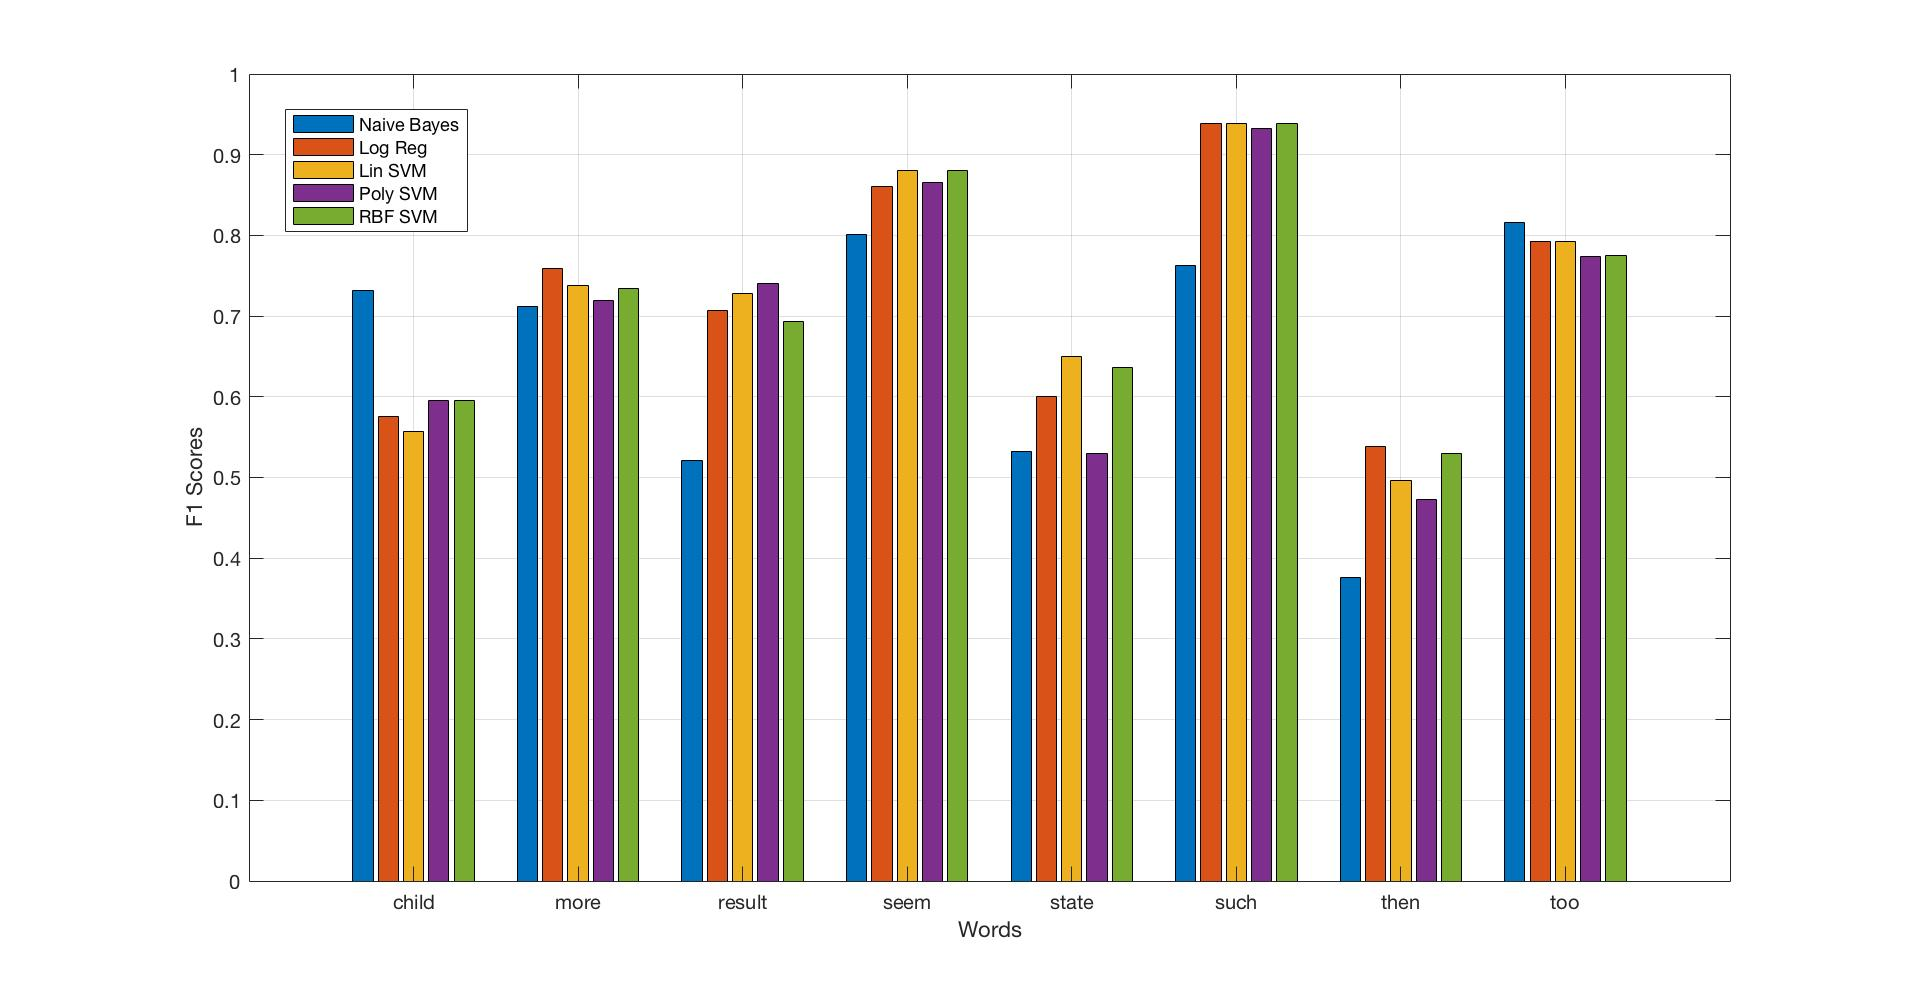
\includegraphics[width=0.7\textwidth]{plots/f1.jpg}
    \caption{Weighted F1 scores on each words}
    \label{fig:results:f1}
\end{figure}

Figure~\ref{fig:results:f1} shows the F1 socres for each classifer,
on each ambiguous word.

\Paragraph{Naive Bayes good at balanced classes}.
Naive Bayes shows high variance in terms of F1 score, compared to other
discriminative classifiers, as shown in figure~\ref{fig:results:f1}.
On word ``child'', Naive Bayes outperforms other discriminative classifiers by
about 16\%.
While on other words like ``result'', its F1 score is lowwer by about 28\%.
The problem is class imbalanced. 
On dataset of ``child'' has a class breakdown to (146,61), while words like
``result'' has a breakdown to (127,63,24).
